%B.H.

%\documentclass[usenatbib,useAMS]{mnras}
\documentclass[galaxies,article,accept,moreauthors,pdftex]{mdpi} 

%\usepackage[]{hyperref}
%\usepackage[all]{hypcap}
%\usepackage{natbib}
%\usepackage[left=2.1cm,top=2cm,right=0.8cm,nohead,nofoot]{geometry}
\usepackage{graphics,epsf}
\usepackage{amsmath}                % American Mathematical Society package
\usepackage{amsfonts}               % American Mathematical Society fonts
\usepackage{amssymb}                % American Mathematical Society symbol
\usepackage{epsfig}                 % EPS figures
%\usepackage{rotating}
\usepackage{graphicx}

%\usepackage{xcolor}
%\definecolor{redak}{rgb}{0.9,0.15,0.05}
%\def \textred{\textcolor{red}}
%\def \textred{\textcolor{red!85!green}}
%\def \textred{\textcolor{redak}}

% =================
\def \kms{~\rm{km~s^{-1}}}
\def \kev{~\rm{keV}}
\def \eV{~\rm{eV}}
\def \cmcub{$\rm{cm}^{-3}$}
\def \msyr{~\rm{M_{\odot}}~\rm{yr^{-1}}}
\def \cm{~\rm{cm}}
\def \s{~\rm{s}}
\def \km{~\rm{km}}
\def \gm{\rm{gm}}
\def \K{~\rm{K}}
\def \g{~\rm{g}}
\def \G{~\rm{G}}
\def \au{~\rm{au}}
\def \erg{~\rm{erg}}
\def \yrs{~\rm{yrs}}
\def \yr{~\rm{yr}}
\def \pc{~\rm{pc}}
\def \kpc{~\rm{kpc}}
\def \etc{$\eta$~Car~}
\def \days{~\rm{days}}
\def \Jy{~\rm{Jy}}
\def \mum{~\rm{\mu m}}
\def \keV{~\rm{keV}}
\def \astrobj#1{#1}
%\def \rmModot{~\rm{M_\odot}}
%\def \rmRodot{~\rm{R_\odot}}
%\def \rmLodot{~\rm{L_\odot}}
\def \sun{\odot}
\def \rmModot{~\rm{M_{\sun}}}
\def \rmRodot{~\rm{R_{\sun}}}
\def \rmLodot{~\rm{L_{\sun}}}
\def \rmMJ{~\rm{M_J}}
\def \rmRJ{~\rm{R_J}}
%\def \rmME{~\rm{M_{\Earth}}}
%\def \rmRE{~\rm{R_{\Earth}}}
\def \rmME{~\rm{M_{\oplus}}}
\def \rmRE{~\rm{R_{\oplus}}}
%%%%%%%%%%%%%%%%%%%%%%%%%%%%%%%%%%%


%%%%%%%%%%%%%%%%%%%%%%%%%%%%%%%%%%% START Journal Abbreviations

\makeatletter
%\newcommand\anchor[2]{#2}% 
%\renewcommand\url{\@dblarg\@url}% 
%\def\@url[#1]{\anchor{#1}}% 

\let\jnl@style=\rmfamily 
\def\ref@jnl#1{{\jnl@style#1}}% 
\newcommand\aj{\ref@jnl{Astron. J.}}%        % Astronomical Journal 
\newcommand\araa{\ref@jnl{Annu. Rev. Astron. Astrophys.}}%  % Annual Review of Astron and~Astrophys 
\newcommand\apj{\ref@jnl{Astrophys. J.}}%    % Astrophysical Journal 
\newcommand\apjl{\ref@jnl{Astrophys. J. Lett.}}     % Astrophysical Journal, Letters 
\newcommand\apjs{\ref@jnl{Astrophys. J. Suppl.}}%    % Astrophysical Journal, Supplement 
\newcommand\ao{\ref@jnl{Appl. Opt.}}%   % Applied Optics 
\newcommand\apss{\ref@jnl{Astrophys. Space Sci.}}%  % Astrophysics and~Space Science 
\newcommand\aap{\ref@jnl{Astron. Astrophys.}}%     % Astronomy and~Astrophysics 
\newcommand\aapr{\ref@jnl{Astron. Astrophys. Rev.}}%  % Astronomy and~Astrophysics Reviews 
\newcommand\aaps{\ref@jnl{Astron. Astrophys. Suppl.}}%    % Astronomy and~Astrophysics, Supplement 
\newcommand\azh{\ref@jnl{AZh}}%       % Astronomicheskii Zhurnal 
\newcommand\baas{\ref@jnl{BAAS}}%     % Bulletin of the~AAS 
\newcommand\icarus{\ref@jnl{Icarus}}% % Icarus
\newcommand\jaavso{\ref@jnl{JAAVSO}}  % The~Journal of the~American Association of Variable Star Observers
\newcommand\jrasc{\ref@jnl{JRASC}}%   % Journal of the~RAS of Canada 
\newcommand\memras{\ref@jnl{MmRAS}}%  % Memoirs of the~RAS 
\newcommand\mnras{\ref@jnl{Mon. Not. R. Astron. Soc.}}%   % Monthly Notices of the~RAS 
\newcommand\pra{\ref@jnl{PhRvA}}% % Physical Review A: General Physics 
\newcommand\prb{\ref@jnl{PhRvB}}% % Physical Review B: Solid State 
\newcommand\prc{\ref@jnl{PhRvC}}% % Physical Review C 
\newcommand\prd{\ref@jnl{PhRvD}}% % Physical Review D 
\newcommand\pre{\ref@jnl{PhRvE}}% % Physical Review E 
\newcommand\prl{\ref@jnl{PhRvL}}% % Physical Review Letters 
\newcommand\pasp{\ref@jnl{PASP}}%     % Publications of the~ASP 
\newcommand\pasj{\ref@jnl{PASJ}}%     % Publications of the~ASJ 
\newcommand\qjras{\ref@jnl{QJRAS}}%   % Quarterly Journal of the~RAS 
\newcommand\skytel{\ref@jnl{S\&T}}%   % Sky and~Telescope 
\newcommand\solphys{\ref@jnl{SoPh}}% % Solar Physics 
\newcommand\sovast{\ref@jnl{Soviet~Ast.}}% % Soviet Astronomy 
\newcommand\ssr{\ref@jnl{SSRv}}% % Space Science Reviews 
\newcommand\zap{\ref@jnl{ZA}}%       % Zeitschrift fuer Astrophysik 
\newcommand\nat{\ref@jnl{Nature}}%  % Nature 
\newcommand\iaucirc{\ref@jnl{IAUC}}% % IAU Cirulars 
\newcommand\aplett{\ref@jnl{Astrophys.~Lett.}}%  % Astrophysics Letters 
\newcommand\apspr{\ref@jnl{Astrophys.~Space~Phys.~Res.}}% % Astrophysics Space Physics Research 
\newcommand\bain{\ref@jnl{BAN}}% % Bulletin Astronomical Institute of the~Netherlands 
\newcommand\fcp{\ref@jnl{FCPh}}%   % Fundamental Cosmic Physics 
\newcommand\gca{\ref@jnl{GeoCoA}}% % Geochimica Cosmochimica Acta 
\newcommand\grl{\ref@jnl{Geophys.~Res.~Lett.}}%  % Geophysics Research Letters 
\newcommand\jcp{\ref@jnl{JChPh}}%     % Journal of Chemical Physics 
\newcommand\jgr{\ref@jnl{J.~Geophys.~Res.}}%     % Journal of Geophysics Research 
\newcommand\jqsrt{\ref@jnl{JQSRT}}%   % Journal of Quantitiative Spectroscopy and~Radiative Trasfer 
\newcommand\memsai{\ref@jnl{MmSAI}}% % Mem. Societa Astronomica Italiana 
\newcommand\nphysa{\ref@jnl{NuPhA}}%     % Nuclear Physics A~
\newcommand\physrep{\ref@jnl{PhR}}%       % Physics Reports 
\newcommand\physscr{\ref@jnl{PhyS}}%        % Physica Scripta 
\newcommand\planss{\ref@jnl{Planet.~Space~Sci.}}%  % Planetary Space Science 
\newcommand\procspie{\ref@jnl{Proc.~SPIE}}%      % Proceedings of the~SPIE 

\newcommand\actaa{\ref@jnl{AcA}}%  % Acta Astronomica
\newcommand\caa{\ref@jnl{ChA\&A}}%  % Chinese Astronomy and~Astrophysics
\newcommand\cjaa{\ref@jnl{ChJA\&A}}%  % Chinese Journal of Astronomy and~Astrophysics
\newcommand\jcap{\ref@jnl{JCAP}}%  % Journal of Cosmology and~Astroparticle Physics
\newcommand\na{\ref@jnl{NewA}}%  % New Astronomy
\newcommand\nar{\ref@jnl{NewAR}}%  % New Astronomy Review
\newcommand\pasa{\ref@jnl{PASA}}%  % Publications of the~Astron. Soc. of Australia
\newcommand\rmxaa{\ref@jnl{RMxAA}}%  % Revista Mexicana de Astronomia y Astrofisica

%% added feb 9, 2016
\newcommand\maps{\ref@jnl{M\&PS}}% Meteoritics and~Planetary Science
\newcommand\aas{\ref@jnl{AAS Meeting Abstracts}}% American Astronomical Society Meeting Abstracts
\newcommand\dps{\ref@jnl{AAS/DPS Meeting Abstracts}}% American Astronomical Society/Division for Planetary Sciences Meeting Abstracts



\let\astap=\aap 
\let\apjlett=\apjl 
\let\apjsupp=\apjs 
\let\applopt=\ao 

\makeatother

%%%%%%%%%%%%%%%%%%%%%%%%%%%%%%%%%%% END Journal Abbreviations

%%%%%%%%%%%%%%%%%%%%%%
\firstpage{1} 
\makeatletter 
\setcounter{page}{\@firstpage} 
\makeatother
\pubvolume{xx}
\issuenum{1}
\articlenumber{5}
\pubyear{2020}
\copyrightyear{2020}
%\externaleditor{Academic Editor: name}
\history{Received: date; Accepted: date; Published: date}
\updates{yes} % If there is an~update available, un-comment this line

%%%%%%%%%%%%%%%%%%%%%%

\Title{ASASSN-13db 2014--2017 Eruption as~an~Intermediate Luminosity Optical Transient}

\newcommand{\orcidauthorA}{0000-0002-7840-0181} % Add \orcidA{} behind the~author's name
\newcommand{\orcidauthorB}{0000-0002-1361-9115} % Add \orcidB{} behind the~author's name
\newcommand{\orcidauthorC}{0000-0003-1288-2461} % Add \orcidC{} behind the~author's name



\Author{Amit Kashi *\orcidA{}, Amir M. Michaelis\orcidB{} and~Leon Feigin\orcidC{}} %Please check accuracy of author names and~affiliation.

\address[1]{
%$^{1}$ \quad
 Department of Physics, Ariel~University, P.O. Box  3, Ariel~4070000,~Israel 
}

\corres{\hangafter=1 \hangindent=1.0em \hspace{-1em} Correspondence: kashi@ariel.ac.il}


\abstract{
The~low mass star ASASSN-13db experienced an~EXor outburst in 2013, which~identified it as~a~Young Stellar Object (YSO). Then, from 2014 to 2017 it had another outburst, longer and~more luminous than the~earlier. We~analyze the~observations of the~second outburst, and~compare it to eruptions of Intermediate Luminosity Optical Transients (ILOTs). We~show that the~decline of the~light curve is almost identical to that of the~V838~Mon, a~prototype of a~type of ILOT known as~Luminous Red Nova (LRN). This~similarity becomes conspicuous when oscillations that are associated with rotation are filtered out from the~light curve of ASASSN-13db. We~suggest that the~eruption was the~result of accretion of a~proto-planet of a~few Earth masses. The~proto-planet was shredded by tidal forces before it was accreted onto the~YSO, releasing gravitational energy that powered the~outburst for $\approx 800 \days$, and~ended in a~$\approx 55 \days$ decline phase. When the~accretion material started depleting the~accretion rate lowered and~the~eruption light curve declined for almost two months. Then it exhausted completely, creating a~sharp break in the~light curve. Another possibility is that the~mass was a~result of an~instability in the~proto-planetary disk that lead to a~large episode of accretion from an~inner viscous disk. We~find that the~variation of the~temperature of the~outburst is consistent with the~surface temperature expected from a~depleted viscous accretion disk. The~2014-2017 outburst of ASASSN-13db may be the~least energetic ILOT to have been discovered to date, with an~energy budget of only $\approx 10^{42} \erg$.
}

\keyword{planet-star interactions ; accretion, accretion discs ; stars: pre-main-sequence ; (stars:) binaries: general}


\begin{document}

%\label{firstpage}
%\pagerange{\pageref{firstpage}--\pageref{lastpage}}
%\maketitle


% ==========================================================
\section{Introduction}
\label{sec:intro}
% ==========================================================

Intermediate luminosity optical transients (ILOTs) are exotic outbursts with luminosities which~fall between those of novae and~supernovae (SN). Many new ILOTs are being discovered by modern surveys and~dedicated campaigns (e.g.,~\cite{Mouldetal1990, Bondetal2003, Rauetal2007, Rauetal2009, Ofeketal2008, Ofeketal2016, Prietoetal2009, Botticella2009, Smithetal2009, Berger2009a, Berger2009b, KulkarniKasliwal2009, Mason2010, Pastorello2010,Pastorelloetal2019a, Pastorelloetal2019b, Kasliwaletal2011, Kasliwal2013, Tylendaetal2013, Kurtenkovetal2015, Smarttetal2015, Williamsetal2015, Ofeketal2016, Pejchaetal2016a, Pejchaetal2016b, Tartagliaetal2016, Villaretal2016, Humphreysetal2017, Humphreysetal2019, Blagorodnovaetal2017, Adamsetal2018, Bellmetal2019, Jayasingheetal2019}. 
 The~group consists of many different astronomical eruptions which~are diverse, but~are found to have shared properties~\citep{Kashietal2010, SokerKashi2016, Kashi2018Galaxies}. Kashi and~collaborators~\cite{Kashietal2010} noticed similarities in the~light curves of a~few ILOTs, that were not considered to be~similar. The~shape of the~light curve may start with a~few peaks (frequently~two~peaks) followed by a~downward concave curve. At~first sight, the~time-scale for decline, and~the~absolute magnitude of the~curve may look different. Their~similarity becomes evident when they are re-scaled, shifting the~peak luminosities to coincide just before the~decline in the~light curve, and~multiplying the~light curves by a~scaling factor.
In \cite{Kashietal2010} it was proposed that this similarity could indicate that a~common physical mechanism is involved, that has a~fingerprint in the~form of this similar decline.


The~Energy-Time Diagram (ETD; \cite{Kashietal2010}, ~\cite{Kashi2018Galaxies})
 is used for classifying transients in terms of their characteristic time of decline and~their total energy (The~ETD webpage: \url{phsites.technion.ac.il/soker/ilot-club/}.). 
 In~the~ETD many of the~transients form a~slated stripe more energetic, for~a~given time scale, than novae yet less energetic than SNe. We~refer to this stripe as~the~Optical Transient Stripe. In~\cite{Kashietal2010} it was suggested that most objects that populate the~stripe share a~similar powering mechanism, that they suggest to be accretion energy. The~different time scale are related to the~accretion rate or the~mass supply rate, that in some cases can be limited by the~time it takes to dissipate the~angular momentum of the~accreted mass through~viscosity.

One well studied transient is the~2002 outburst of V838~Mon~\citep{Bondetal2003}. It~is considered a~prototype of a~sub-type of ILOTs, known as~Luminous Red Novae (LRN). Both classical nova and~He-shell flash were suggested as~explanations for the~unusual eruption, but~later ruled out~\citep{TylendaSoker2006}. The~star involved in the~V838 Mon eruption was a~massive star, possibly even on the~main-sequence (MS). Perhaps~the~most unusual observation was that as~time passed V838~Mon became redder\citep{Evansetal2003,Starrfieldetal2005}, which~is exactly opposite to the~evolution of classical~novae.

A~model for the~eruption of V838~Mon that involves a~stellar merger event followed by an~accretion process, in which~the~surviving star accreted the~material of its destructed companion, was proposed by~\cite{SokerTylenda2006}. The~model was named the~merger-burst model. This~model was able to account for all observations and~its only drawback was that its parameters were not strictly constrained (see~also~\cite{Tylendaetal2005, TylendaSoker2006}). The~binary merger scenario in V838~Mon was strengthened by the~eruption of the~LRN V1309~Sco~\citep{Mason2010} where a~clear signal of an~eclipsing binary was observed prior to the~eruption~\citep{Tylendaetal2011}.

Recently,~\cite{Pastorelloetal2019b} also considered both single star and~binary models for a~collection of LRNe, and~favored a~binary merger model with common envelope ejection. They~made a~distinction for objects fainter than $M_V=-10$, which~they termed Red Novae, and~brighter than this value (typically~at~$M_V=-12$--$-15$), which~they termed Luminous Red Novae. They~suggested that different stellar progenitors are responsible for each of the~two, but~agreed that LRNe are ``scaled-up'' Red Novae. As~we are interested in the~physical mechanism we will not use this~subdivision.

Interestingly,~\cite{Bearetal2011} suggested that merger of a~planet with a~Brown Dwarf or low mass star can lead to an~eruption of shorter time scale and~slightly less energetic, that would be on the~lower left side of the~optical transient stripe. It~later was discovered that some eruptions can have shared properties with ILOTs even if they are external to the~optical transient stripe~\citep{KashiSoker2017, Soker2018}. In~\cite{KashiSoker2017} it was
suggested that the~unusual outburst of the~Young Stellar Object (YSO) ASASSN-15qi~\citep{Herczegetal2016} is an~ILOT event, similar in many respects to LRN events such~as V838~Mon, but~much fainter and~of lower total energy. In~other words, ASASSN-15qi is an~unusual ILOT in the~sense that it has low power and~therefore resides below the~OTS. The~physical model for ASASSN-15qi suggests that in a~similar manner to LRNe, a~secondary object was tidally destroyed onto the~primary YSO, releasing gravitational energy in the~process~\citep{KashiSoker2017}. They~suggested that the~secondary object was a~Saturn-like \textit{planet} instead of a~low mass pre-MS companion in the~LRN model. This~process created an~accretion disk and~manifested as~a~gravitationally powered ILOT. Differently from V838~Mon which~is much more energetic, the~mass of the~destructed planet is too low to cause the~YSO to have an~inflated envelope, and~hence the~merger remnant stays hot, and~therefore does not redden as~the~LRNe.

In~addition to ASASSN-15qi,~\cite{Kashi2018Galaxies} further suggested that another transient, ASASSN-13db~\cite{SiciliaAguilaretal2017}, may also be a~related object. The~variable low-mass star ASASSN-13db was identified by the All Sky Automated Survey for SuperNovae (ASAS-SN; e.g., \cite{Jayasingheetal2019}), after brightening in the~visual by $\approx 4$~mag in September~2013
(\cite{Holoienetal2014, Prietoetal2014, Shappeeetal2014}). The~outburst occurred in an~M5 young star surrounded with a~proto-planetary~disk. FU~Ori outbursts (e.g.,~\cite{HartmannKenyon1996,Audardetal2014} and~references~therein) occur in pre-MS stars, and~are observed as~an~extreme
 change in magnitude with a~slow decline that may last for years. The~spectral type also changes during the~outburst. FU~Ori outbursts can be regarded as~more energetic counterparts of the~EXor class of outburst, of which~EX~Lupis is a~prototype~\citep{Herbig2007}. These are pre-MS variables that show flares of a~few months to a~few years, and~of several magnitudes amplitude, as~a~result of episodic mass accretion~\citep{Herbig1998, Audardetal2014}. The~various intensities and~various timescales are not only found observationally, but~are also expected from theory~\citep{Clarkeetal2005, Zhuetal2009, Vorobyovetal2013}. ASASSN-13db was classified as~an~EXor but~with remarkable luminosity, comparable to EX Lupi 2008 outburst~\citep{Aspinetal2010}, so that it may be a~link between FUors and~EXors~\citep{ContrerasPenaetal2017}.


\textls[-15]{The~2013 outburst was not the~last word heard from ASASSN-13db~\citep{SiciliaAguilaretal2017}. Later, in 2014, ASASSN-13db had another outburst of a~different nature (not an~FU~Ori outburst), in~which~the~peak magnitude in the~$V$-band was brighter by about $1$~mag than the~outburst in~2013. The~entire 2014--2017 transient lasted about~800~days. It~stayed bright at~a~high plateau for about~500~days, experiencing fluctuations of $\delta V \simeq 1$~mag. Later it started gradually declining for another $\approx 250 \days$, which~ended in~2017 with a~fast decline by approximately~2.5 magnitudes over two months (see~Figure~1 of ~\cite{SiciliaAguilaretal2017}).}

\textls[-5]{In~this paper we examine the~possibility that the~2014--2017 outburst of ASASSN-13db (hereafter~A13db1417) was~an~ILOT similar to a~LRN. In~Section~\ref{sec:obs} we discuss its properties in more detail, and~compare it to a~LRN. In~Section~\ref{sec:model} we propose a~model for this outburst. Our~summary and~discussion appear in Section~\ref{sec:summary}.}


% ==========================================================
\section{Observational Comparison}
\label{sec:obs}
% ==========================================================

According to~\cite{Holoienetal2014} ASASSN-13db is an~M5 star with mass $M_1 \sim 0.15 \rmModot$, luminosity $L_1 \simeq 0.06 \rmLodot$ and~radius $R_1 \sim 1.1 \rmRodot$. These values were measured during the~short quiescence phase after the~2013 outburst.
The~distance of ASASSN-13db is estimated to be $\approx 380 \pc$~\citep{SiciliaAguilaretal2017}. We~will adopt these properties in our analysis.

We~focus on the~decline phase of A13db1417.
First, we gathered the~light curves from the~three observatories from where the~data was provided separately in~\citep{SiciliaAguilaretal2017}: ASASSN $V$-band, Beacon $V$-band, and~LCOGT $g'$-band, into one combined light curve. This~will appear later in Figure~\ref{fig:v838_VS_13db} as~``All~ASASSN~13db''. As~evident in the~observations of~\cite{SiciliaAguilaretal2017}, the~decline phase starts at~$V \simeq 14$ and~continues up to the~$V \simeq 18$, in a~generally concave shape. Then, $\approx51$--$59 \days$ after the~peak (there~is a~gap in the~observations that makes it hard to~tell), the~light curve breaks to a~shallow, bumpy~decline.

In~the~study of SNe, it is a~common practice to stretch the~light curves in order to match them (e.g.,~\cite{Goldhaberetal2001,Conleyetal2008}). This~practice is essentially what made possible to derive the~Parker law for SNe Ia, that~allows using them as~standard candles for determining cosmological distances. A~reassembling process was recently suggested for classical novae~\citep{HachisuKato2019}. This~process was used for identifying candidate ILOTs and~comparing between eruptions~\citep{Kashietal2010}, and~developing models for possible new ILOTs (e.g.,~\cite{Bearetal2011}).

To apply this procedure we shifted down the~much more luminous light curve of the~2002 outburst of V838~Mon~\citep{Bondetal2003,Starrfieldetal2005,Sparksetal2008} by $6.9$ mag, to have its peak at~the~same brightness as~that of A13db1417.
We~then superimposed the~light curve of the~outburst of V838~Mon on A13db1417.

Figure~\ref{fig:v838_VS_13db} shows in the~upper panel the~result of only a~simple shift, for which~the~second peak before the~decline (one before last) was matched for both transients.
The~two transients show a~similar decline for about 3 magnitudes.
The~light curves of the~two transients separate only after this shared decline, as~A13db1417 at~this point has a~bump in the~light curve (JD$\simeq2457779$, which~is $\simeq50 \days$ after the~last peak before decline).
On~the~lower panel, we matched the~peak just before the~decline starts. We~find that when the~time axis of the~light curve of V838~Mon is scaled by a~factor of 1.3 the~two light curves behave similarly for a~decline of $\Delta V \simeq 4$~mag.

A~period of $\sim$4.2 days superimposed in the~light curve of A13db1417 was found by~\cite{SiciliaAguilaretal2017}. Their~explanation for that periodicity, which~can even be seen by visually examining the~data, was~stellar rotation and~the~presence of spots. We~wish to filter out this effect from the~data, as~we believe that this effect contaminates a~light curve that is governed by accretion. We~note that we filter out the~variation regardless of its source, may it be spots, binary interaction or a~different~source.

The~A13db1417 signal includes high rate temporal sampling, sometimes a~few times per night and~on other times one measurement per a~few days. We~analyze the~unequally spaced signal power spectrum using the~generalized Lomb-Scargle periodogram (GLSP;~\cite{ZechmeisterKurster2009}), and~obtain a~wealth of high frequencies in the~power spectrum. We~use the~following method to transfer A13db1417 unevenly spaced data to a~per night regular sampled signal. We~first focus on the~data points that were sampled more than once at~a~night and~decimate the~signal using simple average result with a~per night data point. Then we use spline interpolation on the~signal to estimate the~missing data points. This~results in a~regular sampled signal per night. We~compare the~GLSP analysis with our new regular signal using Welch method~\citep{Welch1967} as~well as~the~GLSP (setting the~relevant parameters to evenly spaced sampling) power spectrum making sure we did not lose information (mainly more than 4 days periods).  As~a~final step we apply the~median filter (again~after checking with the~power spectrum and~making sure we do not lose information) to~emphasize the~signal trend behavior over the~fast temporal~fluctuation.

%FFFFFFFFFFFFFFFFFFFFFFFFFFFFFFFFFFFFFFFFFFFFFFFFFFFFFFFFFFFFFFFFFFF
\begin{figure}[t]
\centering
\begin{tabular}{c}
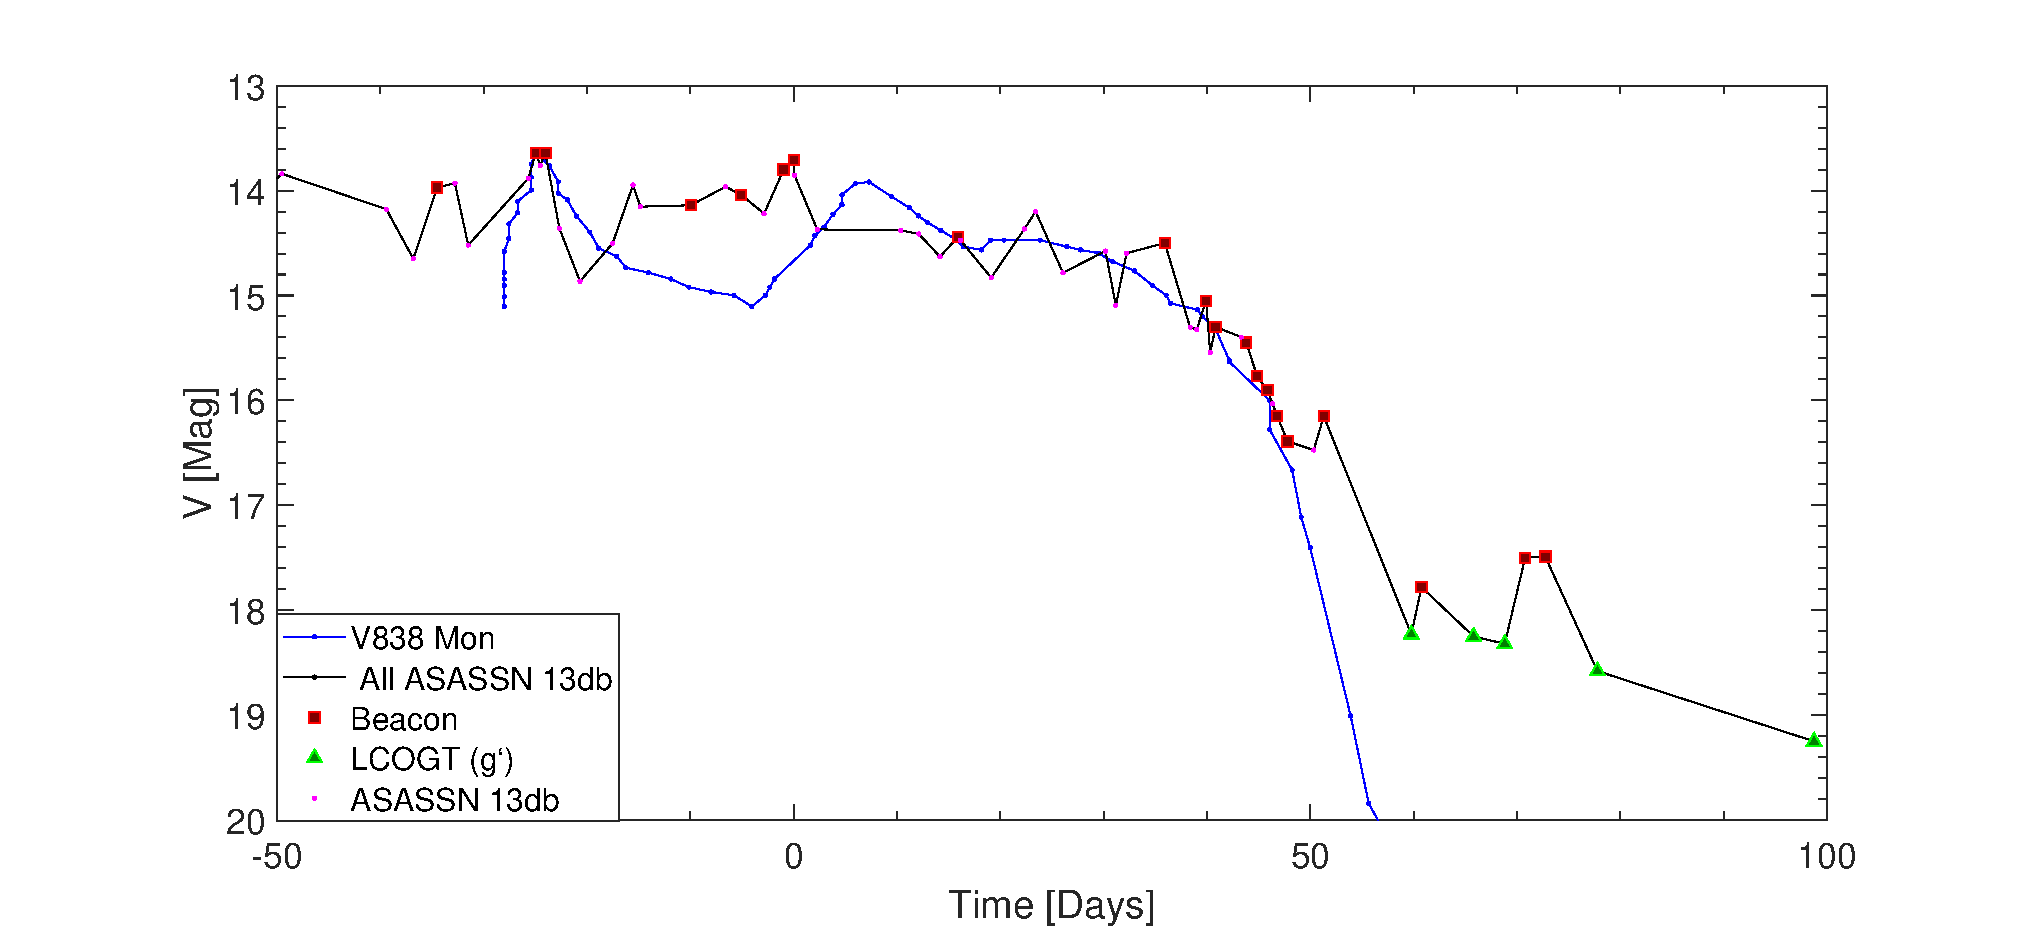
\includegraphics[trim= 0.9cm 1.5cm 1.0cm 0.8cm,clip=true,width=0.9\textwidth]{All11.eps}\\
(\textbf{a}) \\ % l b r t
\includegraphics[trim= 0.9cm 0.0cm 1.0cm 0.8cm,clip=true,width=0.9\textwidth]{ALL10.eps}\\
 % l b r t
%\includegraphics[trim= 0.9cm 0.0cm 1.0cm 0.0cm,clip=true,width=0.5\textwidth]{pp.eps}
(\textbf{b}) \\
\end{tabular}
\caption{\textls[-15](\textbf{a}) Comparing the~$V$-band light curves of A13db1417~\citep{SiciliaAguilaretal2017} and~V838~Mon (\cite{Bondetal2003, Starrfieldetal2005,Sparksetal2008}). The~magnitude scale is the~apparent magnitude for A13db1417. The~light curve of V838~Mon was shifted by $\Delta V_{\rm V838~Mon} =6.9$~mag to match the~second peak before decline. The~time axis  focuses on the~end of the~$\approx 800 \days$ duration of A13db1417 (see \cite{SiciliaAguilaretal2017}) which~is the~$\simeq 55 \days$ decline phase. The~peak at~$\rm{JD} \simeq 2457728$ marks $t=0$. (\textbf{b}) Same us the~upper panel, but~the light curves were shifted to match the~peak just before decline. In~addition, the~time axis of the~light curve V838~Mon is scaled by a~factor of 1.3 relative to the~matched peak. This~results in that the~two light curves match for about~4~mag. %6.8665 
}
\label{fig:v838_VS_13db}
\end{figure}
%FFFFFFFFFFFFFFFFFFFFFFFFFFFFFFFFFFFFFFFFFFFFFFFFFFFFFFFFFFFFFFFFFFF

Figure~\ref{fig:v838_VS_13db_filtered} shows the~results of this process.
The~obtained light curve is much more refined and~less bumpy than the~original.
Therefore, much more resembling the~smooth decline light curve of V838~Mon.
We~can see~that as~expected the~two light curves match much~better.


%FFFFFFFFFFFFFFFFFFFFFFFFFFFFFFFFFFFFFFFFFFFFFFFFFFFFFFFFFFFFFFFFFFF
\begin{figure}[t]
\centering
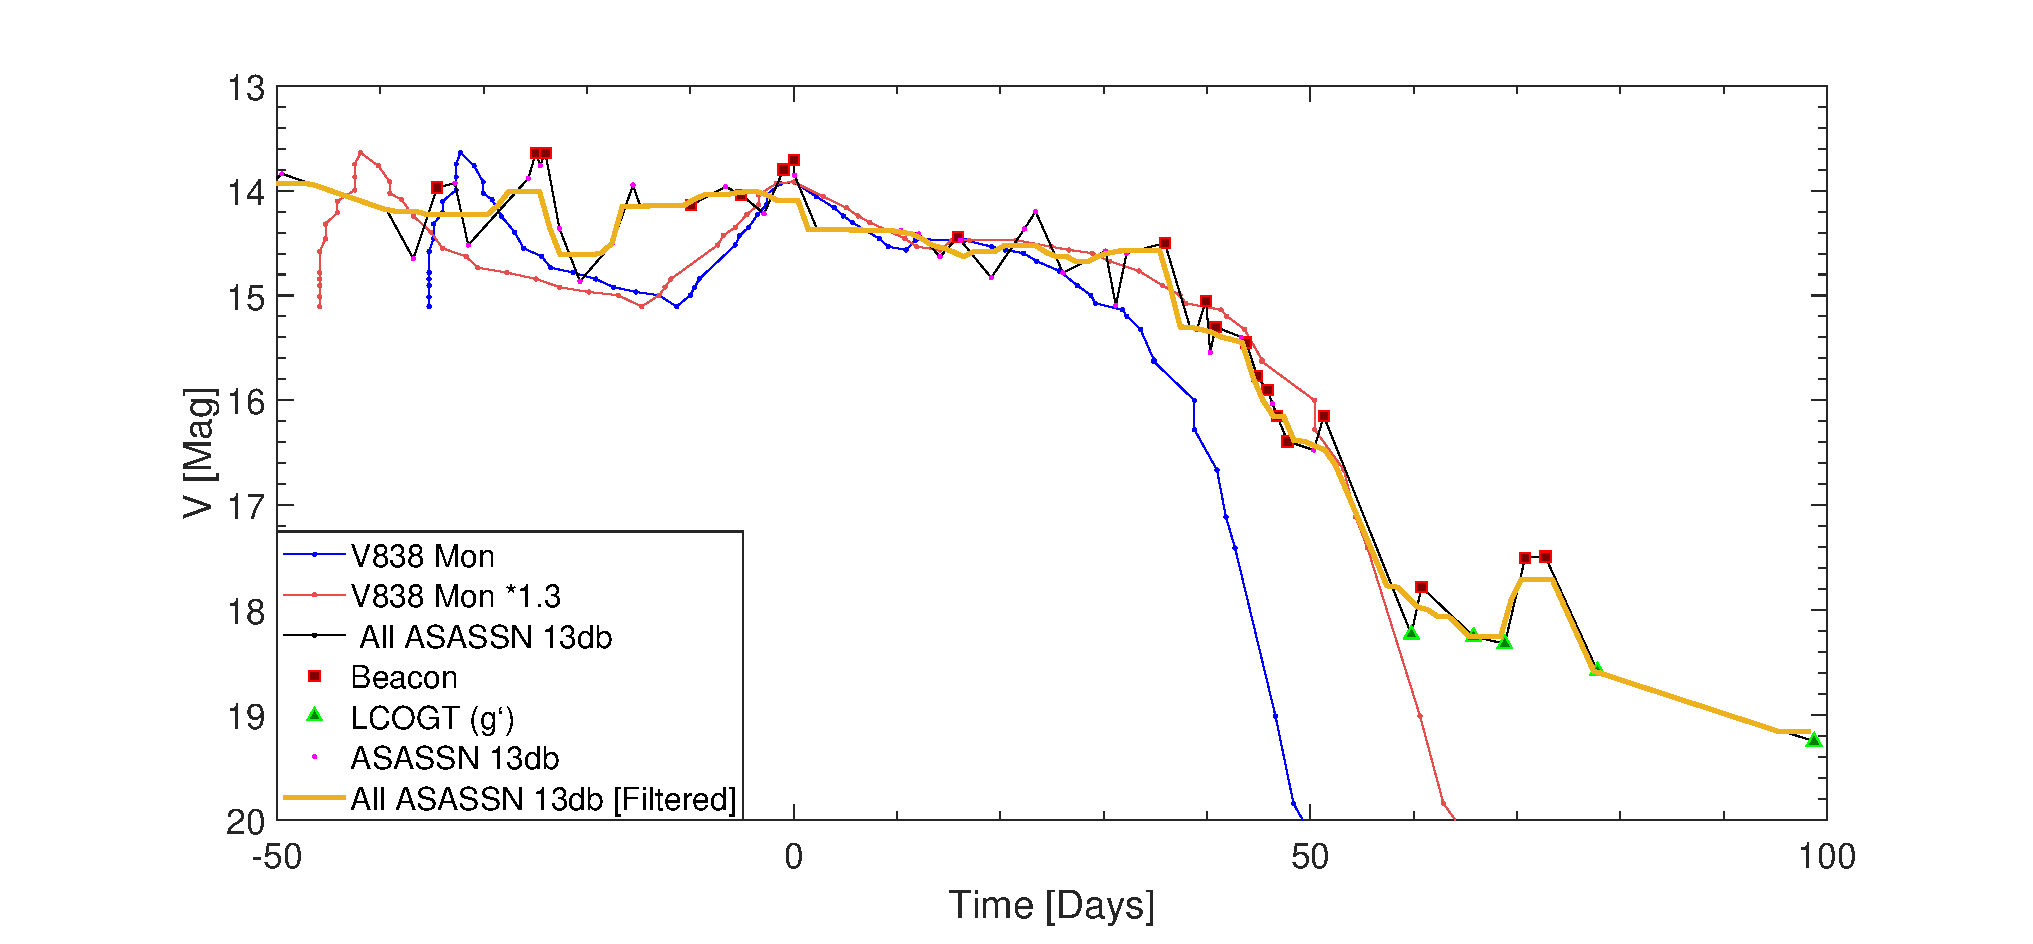
\includegraphics[trim= 0.9cm 0.0cm 1.0cm 0.8cm,clip=true,width=0.9\textwidth]{ALL9.eps} % l b r t
\caption{The~light curve of A13db1417, with the~variability resulted by rotation of stellar spot filtered out, compared to the~light curve of V838~Mon. This~variability caused oscillations of $\delta V \simeq 1$~mag. By~filtering out the~effect of rotation, we isolate the~component resulted from accretion.
The~filtered signal matches better the~scaled light curve of V838~Mon.}
\label{fig:v838_VS_13db_filtered}
\end{figure}
%FFFFFFFFFFFFFFFFFFFFFFFFFFFFFFFFFFFFFFFFFFFFFFFFFFFFFFFFFFFFFFFFFFF

According to~\cite{SiciliaAguilaretal2017}, the~light curve of A13db1417 has an~overall shape that strongly resembles in length, duration, and~general shape (including~the~quick magnitude
drop after a~slow fading) the~light curve of the~FU~Ori variable V1647~Ori that erupted in 2004 (\cite{Fedeleetal2007}~and references therein). The authors of \cite{SiciliaAguilaretal2017} did not, however, present any comparison of these two light~curves. Reference~\cite{Fedeleetal2007} do not bring $V$-band observations of V1647~Ori, but~rather $R_c$-band covering well the~outburst and~its decline. In~Figure~\ref{fig:V1647Ori} we~compare the~$R$-band/$r'$-band light curve of A13db1417 with the~$R_c$-band of V1647~Ori. As~there are no ASASSN $R$-band observations, but~the~observations from Beacon and~LCOGT show thar $R-V$ and~$r'-g'$ are almost constant, we~adopt a~constant shift of $V-R=0.8$ for the~ASASSN observations, and~use its $V$-band observations to obtain the~$R$-band. We~evaluate the~error in this method is~$\pm 0.1$~mag.  Figure~\ref{fig:V1647Ori} shows that, though we try to make the~two light curves match, the~two objects have quite different decline slopes, with that of V1647~Ori being much steeper. The~comparison to V838~Mon is by far superior. We~consider it to be another hint that A13db1417 is not an~FU~Ori~eruption.



%FFFFFFFFFFFFFFFFFFFFFFFFFFFFFFFFFFFFFFFFFFFFFFFFFFFFFFFFFFFFFFFFFFF
\begin{figure}[t]
\centering
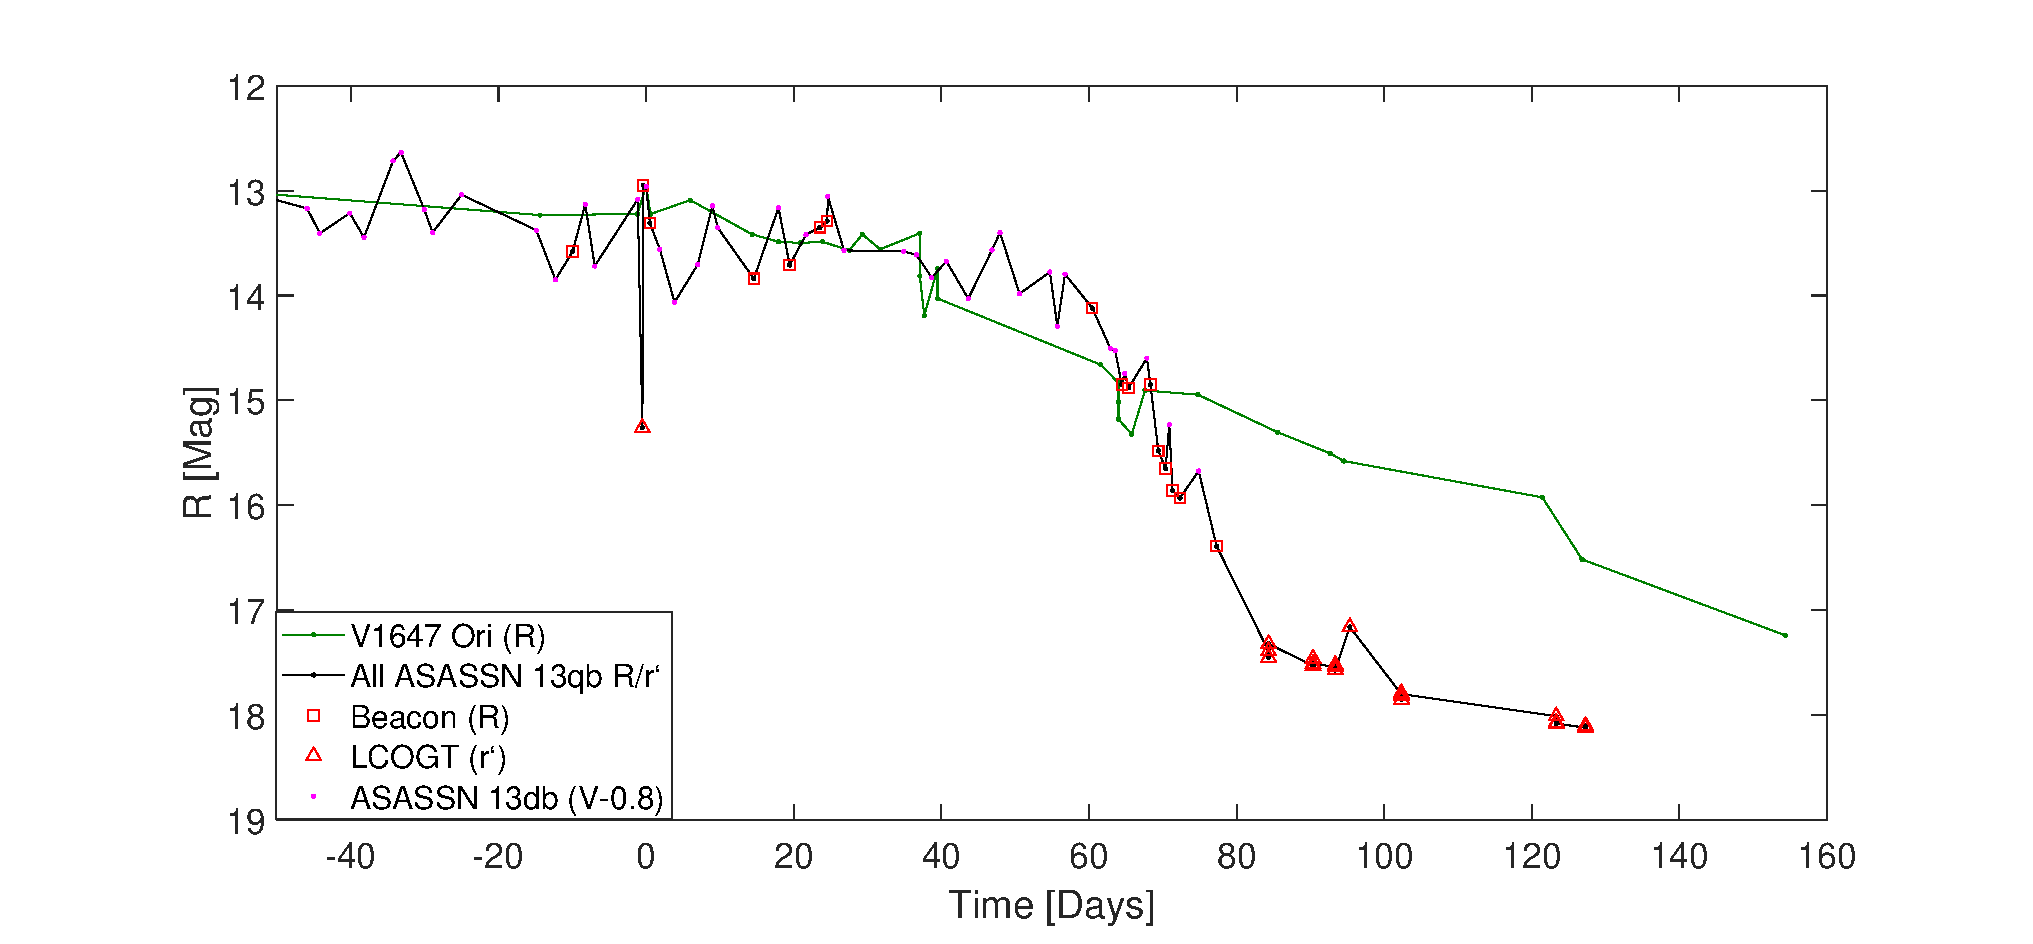
\includegraphics[trim= 0.9cm 0.0cm 1.0cm 0.8cm,clip=true,width=0.9\textwidth]{V1647_4.eps} % l b r t
\caption{\textls[-12]{The~light curve of A13db1417 compared to that of the~FU~Ori eruption of V1647~Ori~\citep{Fedeleetal2007}. It~can be seen that the~two curves are very different and~the~decline does not follow the~same slope. This~suggest that this objects are different. Note that the~LCOGT observation at~$t=-2 \days$ may be an~outlier.}
%%%This~may be another indication that A13db1417 is not an~FU~Ori eruption, as~those have typically a~steeper slope.
}
\label{fig:V1647Ori}
\end{figure}
%FFFFFFFFFFFFFFFFFFFFFFFFFFFFFFFFFFFFFFFFFFFFFFFFFFFFFFFFFFFFFFFFFFF
We~calculate the~temperature from the~available observations, but~the~observations are quite noisy, and~when calculating color the~noise does not cancel. The~results during the~decline show that the~effective temperature slowly declines with time during the~55 days of disk dissipation (Figure~\ref{fig:Tt}). The~observations are insufficient for performing detailed comparison. However, we can compare them to the~evolution of the~effective temperature of V838~Mon (see~figure 2 in~\citep{Tylenda2005}). We~can see~that both objects had their effective temperature declining from $\simeq 4500\K$ to $\simeq 2000\K$ during the~eruption, a~similarity that adds to the~similarity in the~light curve we showed~above.

%FFFFFFFFFFFFFFFFFFFFFFFFFFFFFFFFFFFFFFFFFFFFFFFFFFFFFFFFFFFFFFFFFFF
\begin{figure}[t]
\centering
\includegraphics[trim= 0.0cm 0.0cm 0.0cm 0.0cm,clip=true,width=0.9\textwidth]{T-JD-V838} % l b r t
\caption{The~effective temperature of A13db1417, obtained from different filters as~indicated in the~legend. The~calculation was performed assuming black-body emission, which~is apparently not the~emitting spectrum, hence the~differences between the~estimated in different filter pairs.
Nevertheless we can see~that the~effective temperature is declining from $\simeq 4500\K$ to $\simeq 2000\K$ during the~eruption. Over-plotted is the~effective temperature from of V838~Mon, adopted from~\citep{Tylenda2005}. It~is evident that both objects have a~similar decline. }
\label{fig:Tt}
\end{figure}
%FFFFFFFFFFFFFFFFFFFFFFFFFFFFFFFFFFFFFFFFFFFFFFFFFFFFFFFFFFFFFFFFFFF



% ==========================================================
\section{An~ILOT Model}
\label{sec:model}
% ==========================================================

In~Section~\ref{sec:obs} we showed that the~characteristic decline of the~light curve of A13db1417 was similar to that of  V838~Mon. We~adopt the~model of~\cite{SokerTylenda2006} that suggests that a~merger event lead to the~outburst of V838~Mon. In~\cite{SokerTylenda2006} it was estimated that the~eruption of V838~Mon involved ejecting mass with kinetic energy of $E_{\rm kin} \approx 10^{44} \erg$, which~is about an~order of magnitude larger than the~emitted radiated energy of the~eruption. As~mentioned earlier in Section~\ref{sec:intro}, in~\cite{KashiSoker2017} the~properties of the~YSO eruption ASASSN-15qi were compared to those of V838~Mon. The~merger-like scenario that they suggested involved a~secondary object that was tidally destroyed onto the~primary $\approx 2.4 \rmModot$ YSO, releasing gravitational energy in the~process.
They~estimated that the~ejected mass could have a~similar value for the~kinetic energy, $E_{\rm kin} \approx 10^{44} \erg$.

We~now turn to examine a~model in which~A13db1417 was a~result of a~destruction of a~proto-planet onto the~YSO. The~innermost proto-planetary disk gas can be drained during the~previous EXor outburst, creating a~``disk gap'' (e.g.,~\cite{Gotoetal2011,BanzattiPontoppidan2015}). But~then in~2014 the~planet arrives and~shredded into fragments that from a~temporary disk, that exists until its depletion in~2017. Such~a~destruction would be the~result of instabilities in the~proto-planetary disk that may contain a~number of large bodies that interact with each other and~with the~material in the~proto-planetary disk. If~such an~object comes into the~tidal destruction radius of the~YSO, it~would be shredded and~form an~accretion disk. The~material would fall onto the~star, releasing gravitational energy. The~process would continue until the~available material is depleted, after~which~the~light curve would decline. It~is also possible, as~we discuss below, that the~instability in the~disk causes accretion of material in the~form of gas rather than a~destructed planet. It~is only required that the~arriving material would posses enough angular momentum to form a~close accretion disk around the~proto-star.

Modeling the~observations of A13db1417,~\cite{SiciliaAguilaretal2017} suggested accretion rates $\lesssim 3 \times 10^{-7} \msyr$. It~is not mentioned, however, whether this estimate includes the~kinetic energy (Namely, it was not mentioned whether the~supply of the~accreted gas can account only for radiation or for all the~energy). The~radiated energy during the~$\approx 800$ days of A13db1417 is $E_{\rm rad} \approx 2\times 10^{41} \erg$. The~wings of the~H$\alpha$ line observed in A13db1417 reach $300 \kms$~\cite{SiciliaAguilaretal2017}, indicating the~gas reach that velocity. We~will calibrate the~calculations of the~energy with $v_{\rm ej}=300 \kms$.
The~kinetic energy involved in the~eruption of A13db1417 can therefore be calibrated~as
\begin{equation}
E_{\rm kin} \simeq 9 \times 10^{41}
\left(\frac{M_{\rm ej}}{10^{-6}\rmModot}\right)
\left(\frac{v_{\rm ej}}{300 \kms}\right)^2 \erg, % 8.955
\label{eq:Ekin}
\end{equation}
where $M_{\rm ej}$ is the~ejected mass. A~lower velocity would result smaller energy, but~as~most of the~mass probably travels in the~range of $\gtrsim 100 \kms$, the~energy should still be in the~range of few $\times 10^{41} \erg$. As~the~accreted mass is small, we do not expect the~envelope to inflate, a~process that may consume more energy, which~is not observed. Namely the~total energy involved in the~A13db1417 eruption is $E_{\rm tot} \approx 10^{42} \erg$.
The~gravitational energy that can be supplied through accretion of a~total amount of mass $M_{\rm acc}$ from a~destructed object can be calibrated with the~parameters of the~YSO as
\begin{equation}
E_{\rm grav} \simeq 2.6 \times 10^{42}
\left(\frac{M_1}{0.15\rmModot}\right)
\left(\frac{M_{\rm acc}}{10^{-5}\rmModot}\right) 
\times \left(\frac{R_1}{1.1 \rmRodot}\right)^{-1} \erg. \\ %2.58857 
\label{eq:Erad}
\end{equation}
Namely, the~accreted object has the~mass of a~planet, possibly a~proto-super-earth planet with mass of few $\times 10^{-6}$--$ 10^{-5}\rmModot$. The~average accretion rate we obtain over the~$t_{\rm acc} \approx 800 \days$ of the~eruption~is
\begin{equation}
\dot{M}_{\rm acc} \simeq 4 \times 10^{-6}
\left(\frac{M_p}{3 \rmME}\right) \left(\frac{t_{\rm acc}}{800 \days}\right)^{-1} \msyr. % 0.000004113
\label{eq:mdotacc}
\end{equation}
This~value (for the~accretion rate during the~outburst) is about 3000 times larger than the~quiescence accretion rate from the~proto-planetary disk, obtained from spectroscopic lines~\citep{SiciliaAguilaretal2017}. It~might be that the~mass is supplied not from a~proto-planet but~rather directly from the~proto-planetary disk, that~due~to an~instability increases the~accretion rate for the~duration of the~eruption. In~this case an~inner denser disk may from (or~a~thicker disk-like structure) that contains the~mass that was transferred from the~protoplantary disk to the~star, while it is being consumed by the~proto-star.

The~radii of proto-planets depend on their age, the~size of the~core, the~accretion rate onto the~core (if they are created by accretion of planetesimals), the~planet pressure profile, and~the~efficiency of cooling with the~presence (or~obscuration) of stellar irradiation and~tidal heating (e.g., \cite{Baruteauetal2016, Fortneyetal2007, Guillot2005} and~references~therein). According~to these studies, at~a~young age the~radius can be twice or more the~final radius. \cite{Fortneyetal2007} emphasize that planets that form closer to their star have a~larger radius, especially at~young ages.
Therefore the~expected density of a~proto-super-earth~is

\begin{equation}
\rho_p \simeq 1.06
\left(\frac{M_p}{3 \rmME}\right)
\left(\frac{R_p}{2.5 \rmRE}\right)^{-1}~\rm{g~cm^{-3}}, %2.062 %1.0557
\label{eq:rho_p}
\end{equation}
where $M_p$ and~$R_p$ are the~planet mass and~radius, respectively.

We~would like to clarify that when we use the~name super-earth we do not necessarily mean that the~planet is of a~rocky nature. We~only use this term to make a~connection to the~mass of the~planet we discuss. It~may well be a~that this planet is gaseous, and~the~exact composition does not make a~significant difference to the~applicability of our model. Indeed, a~peculiar composition will reflect in the~observed spectra, but~we expect the~accreting object to have formed from the~very same cloud that formed the~YSO, so their composition should be~similar. 

The~Roche limit for tidal destruction of such a~proto-planet is
\begin{equation}
r_d \approx 2.44 \left( \frac{\rho_1}{\rho_p} \right)^{1/3} R_1
\approx 1.43
\left(\frac{\rho_1}{0.16~\rm{g~cm^{-3}}}\right)^{1/3}
\left(\frac{\rho_p}{1.06~\rm{g~cm^{-3}}}\right)^{-1/3}
\times \left(\frac{R_1}{1.1 \rmRodot}\right) \rmRodot \\ %1.4274 % 2.44*0.585
\label{eq:r_d}
\end{equation}
where $\rho_1$ is the~density of the~YSO, calculated based on the~parameters derived by~\citep{SiciliaAguilaretal2017}. The~proto-planet is likely to have approached to the~YSO in a~grazing angle, due to an~instability in the~proto-planetary disk. As~Roche limit is larger than the~YSO radius, the~proto-planet would be destructed as~it comes closer to the~YSO by its gravitational field even though its average density is~larger.

Close to the~end of the~$\approx 800 \days$ of accretion, once the~mass supply from the~shredded proto-planet material is terminated, there is an~accretion disk (could be a~thick disk) left that will exhaust itself on a~viscosity timescale.
\begin{equation}
t_{\rm{visc}} \simeq \frac{R_1^2}{\nu} \simeq 55
\left(\frac{\alpha}{0.1}\right)^{-1}
\left(\frac{H/R_a}{0.1}\right)^{-1}
\left(\frac{C_s/v_\phi}{0.1}\right)^{-1}
\times
\left(\frac{R_1}{1.1 \rmRodot}\right)^{3/2}
\left(\frac{M_1}{0.15 \rmModot}\right)^{-1/2} ~\rm{days}, %6.0751*12=72.9012   %72.9*0.7536=54.94
\label{eq:tvisc1}
\end{equation}
where $H$ is the~thickness of the~disk, $C_s$ is the~sound speed, $\alpha$ is the~disk viscosity parameter, $\nu=\alpha ~C_s H$ is the~viscosity of the~disk, and~$v_\phi$ is the~Keplerian velocity.
We~get that \textit{$t_{\rm{visc}}$ matches the~time of the~break in the~light curve, discussed above}. This~may indicate that for $\approx2$ months the~light curve is governed (other~than the~contamination from the~rotating spot) by the~depletion of the~accretion disk that the~proto-planet~created. Then comes the~break in the~light curve and~a~shallower decline in brightness.

In~the~above calculation we used a~constant accretion radius of $1.1 \rmRodot$.
Spectral analysis of A13db1417, that found many lines to have inverse P~Cygni or YY~Ori type profiles, lead~\cite{SiciliaAguilaretal2017} to conclude that: (1)~The~YSO and~its proto-planetary disk are viewed almost edge-on. (2)~The~effective temperature during the~eruption is lower than at~quiescence.

We~estimate the~Keplerian time at~the~destruction radius to be $t_k \simeq 0.5 (r_d / 1.4 \rmRodot)^{3/2} \days$. %0.4956
The~ratio of viscous to Keplerian timescale is $t_{\rm{visc}}/t_K \simeq 110$. Therefore as~the~accreted material from the~planet is destructed onto the~YSO, it might create a~\textit{thick} accretion~disk.


Let us discuss the~beginning of A13db1417. At~the~beginning of the~$\approx 800 \days$ outburst, a~planet is destructed. The~fall-back time for mass to start being accreted is about 6 days for the~parameters we adopted/derived.
%Td~(pi/Mp)*(Ms*Rp^3/(2*G))^(1/2)~6 days
Very quickly, in a~matter of a~few dynamical times (namely a~few days) most~of the~destructed material which~falls with a~non-zero angular momentum, will form an~accretion disk. Therefore we expect, and~indeed there is, a~steep increase in the~luminosity. Figure~\ref{fig:beginning} focuses on the~beginning on the~outburst, showing its fast increase in brightness. As~a~characteristic observational constraint to the~increase in the~luminosity at~the~beginning of A13db1417, we~take the~time from the~first detection to the~first local peak, which~about $13 \days$. This~time scale can give a~rough estimate to the~transition time from the~fal-lback accretion, for which~the~destruction time scale is the~relevant timescale, and~the~viscous accretion. We~emphasize that the~source of the~luminosity during the~remainder of the~$\approx 800 \days$ is not from the~destruction itself, but~rather from continuous accretion of the~mass of the~planet onto the~star. It~is therefore possible to very crudely constrain the~fall-back time scale to $\approx 13 \days$, which~is in agreement with the~fall-back time and~the~onset of the~viscous accretion disk.

%FFFFFFFFFFFFFFFFFFFFFFFFFFFFFFFFFFFFFFFFFFFFFFFFFFFFFFFFFFFFFFFFFFF
\begin{figure}[t]
\centering
\includegraphics[trim= 0.0cm 0.0cm 0.0cm 0.0cm,clip=true,width=0.9\textwidth]{figure5.pdf} % l b r t
\caption{A~focus on the~fast increase in luminosity at~the~beginning of A13db1417.
Observations are taken from~\cite{SiciliaAguilaretal2017}.}
\label{fig:beginning}
\end{figure}
%FFFFFFFFFFFFFFFFF


While the~disk exists it may reduce the~number of ionizing photons escaping from the~YSO close to the~equator, and~also lower the~effective temperature. If~the~YSO, is observed from, or close to, an~edge-on line of sight, this will be evident in the~spectra. Therefore we suggest that the~ILOT model can also account for the~variation in the~observed line~intensities.


Analyzing the~data, we find that the~effective temperature of A13db1417 declined from $\simeq$$4500\K$ to $\simeq$$2000\K$ during the~last stage of the~eruption. The~trend and~the~values are similar to the~effective temperature from of V838~Mon~\citep{Tylenda2005}. According~to our model, the~emission of A13db1417 comes from a~viscous disk. Modeling the~emission in our specific case would require an~extensive numerical study, that might be too excessive given the~rough estimate of the~parameters. But~for a~crude estimate, we~calculate the~temperature for a~classical accretion disk~model
\begin{equation}
T(R)=\left( \frac{3 G M_1 \dot{M}_{\rm acc} }{8 \pi R^3 \sigma} \left[1-\left(\frac{R_1}{R}\right)^{1/2}\right] \right)^{1/4}
\label{eq:TR}
\end{equation}
where $R$ is the~disk radius and~$\sigma$ is the~Stefan-Boltzmann constant. Figure~\ref{fig:Tt} shows the~surface temperature for the~disk according to Equation~(\ref{eq:TR}). As~the~disk depletes during \vspace{2pt} the~$\approx 55 \days$, the~mass accretion rate~drops. Consequently, the~temperature drops as~$T \sim \dot{M}_{\rm acc}^{1/4}$.
%The~spectrum of a~classical disk is not exactly a~Planck function but~rather a~similar curve with a~flat top, but~for the~accuracy needed in this calculation, a~simple Plank function is sufficient.
The~outer part of the~disk, that has the~largest surface area and~thus dominant in the~spectrum, has a~surface temperature in the~range of $\simeq3500$--$4500\K$. During the~decline in the~emission of the~outburst drops by $\Delta V \simeq 4$~mag in $\approx 55 \days$ (see~Figure~\ref{fig:v838_VS_13db}), corresponding to a~drop in the~brightness by a~factor of $\simeq40$. Therefore, according to the~model, $\dot{M}$ needs to drop by that factor as~well. As~the~accretion rate drops by that factor of 40 the~temperature drops by a~factor of $\simeq2.5$. We~note that Equation~(\ref{eq:TR}) describes a~steady state and~does not accurately account for the~thermal changes during the~dynamic phase of the~depletion. Given the~crude estimate, it turns out that the~disk surface temperature is consistent with the~observations that show a~surface temperature drop to $\approx2000\K$ at~the~end of the~outburst (Figure~\ref{fig:TR}).

%
%FFFFFFFFFFFFFFFFFFFFFFFFFFFFFFFFFFFFFFFFFFFFFFFFFFFFFFFFFFFFFFFFFFF
\begin{figure}[t]
\centering
\includegraphics[trim= 0.0cm 0.0cm 0.0cm 0.0cm,clip=true,width=0.9\textwidth]{figure6.pdf}
%{temp_r_Mdot_change_3.eps} % l b r t
\caption{An~estimate to a~classical accretion disk surface temperature, according to Equation~(\ref{eq:TR}). When~the~disk is depleted the~mass accretion rate decreases and~so does the~surface temperature of the~disk.}
\label{fig:TR}
\end{figure}
%FFFFFFFFFFFFFFFFFFFFFFFFFFFFFFFFFFFFFFFFFFFFFFFFFFFFFFFFFFFFFFFFFFF

% ==========================================================
\section{Summary and~Discussion} 
\label{sec:summary}
% ==========================================================

We~discussed the~eruptions of the~YSO ASASSN-13db, which~erupted twice: a~short eruption in~2013, and~a~longer one from~2014 to~2017. The~2013 event is a~typical YSO outburst, but~the~2014--2017 event (A13db1417) is clearly different. The~object may be intermediate between FUor and~EXor outbursts. It~has been proposed that there is a~continuous spectrum of variables between EXors and~FUors~\citep{ContrerasPenaetal2017}, based on the~outburst ranges, so~that some bursts may be more FUor-like and~some others more EXor~like.

We~found a~strong resemblance in the~decline light curves of A13db1417 and~V838~Mon, a~prototype LRN ILOT. The~two outburst have similar decline in their light curves, which~we suggest may not be a~coincidence. Namely, we follow~\cite{Kashietal2010} who suggested that mass accretion that releases energy in a~specific rate can account for a~special shape of light curve, that will be similar for different objects when rescaled. There~is also a~similar decline in the~effective temperature of the~two transients. The~evolution of the~temperature also matches the~expected decline of the~surface temperature of a~classical accretion disk, as~a~result from a~decrease in the~accretion rate. Therefore we examine the~possibility that A13db1417 is an~accretion-powered event, as~was suggested for V838~Mon. We~found that the~time from the~peak of the~light curve of A13db1417, to~the~break were it begins a~much shallower decline is the~same as~the~viscosity time on which~the~shredded proto-planet is accreted, and~therefore the~supply of mass for gravitational energy to power the~event is~consumed.

Most stars are expected to form planets at~some point, and~during this process the~orbits are in many cases unstable, what may lead to a~collision course between the~proto-planet and~the~proto-star. We~examined the~possibility that A13db1417 was caused by accretion of a~proto-planet onto the~proto-star, in what is termed an~Intermediate Luminosity Optical Transient~(ILOT).

It~is possible that the~A13db1417 eruption is accretion not from a~destructed planet but~rather of gas from the~proto-planetary disk. The~amount of accreted mass in this case would be the~same as~calculated in Section~\ref{sec:model}, from the~energy considerations. In~that case there should be an~instability in the~proto-planetary disk, that would increase the~normal mass accretion rate to a~few $\times 10^{-6} \msyr$ (see~Equation~(\ref{eq:mdotacc})). If~ASASSN-13db will have more eruptions with the~same declining slope it will be in favor of the~instability in the~proto-planetary disk scenario, as~it is less likely that a~number of planets will interact with the~YSO in the~same manner. The~proto-planetary disk, on the~other hand, does not have such a~constraint, and~multiple instabilities that may lead to eruptions are~possible.

In~Section~\ref{sec:model} we estimated that the~total energy involved in the~A13db1417 eruption is $ \approx 10^{42} \erg$. If~the~outburst is indeed an~ILOT, A13db1417 is the~least energetic one observed to date. The~Eddington ratio for A13db1417 is $\Gamma_{\rm Edd} \simeq 10^{-4}$, which~is very small compared to objects in the~OTS, that can reach even $\Gamma_{\rm Edd} \simeq 10$. %0.000106
It~is therefore located at~the~bottom of the~Energy Time Diagram (ETD), as~a~very weak eruption in terms of energy (as~low as~the~energy of novae and~below), and~an~intermediate duration in the~scale of~months.

\textls[-10]{ASASSN-13db is an~important contribution to the~ILOT family, as~it expands the~region on the~ETD where ILOTs can reside. We~see~that an~ILOT can be not ``intermediate'', in~the~sense that its luminosity does not necessarily be in the~gap between novae and~SNe. The~word ILOT does not classify an~object in terms of its brightness, but~rather designates an~object with a~specific physical process, accretion~and~release of gravitational~energy.}

The~light curve of V838~Mon itself, which~was used here as~a~reference is not yet completely understood. It~was suggested to be the~result of the~merger-burst process, and~was qualitatively obtained from analytic considerations, but~further investigation is~required. An~different interpretation of the~light curve of the~prototype LRN, V838~Mon, as~a~sequence of three planet collision with the~a red giant was proposed by~\cite{RetterMarom2003} and~\cite{Retteretal2006}. Setting aside the~fact that the~progenitor of V838~Mon was not a~red giant, the~scenario they proposed could not account for the~energy of the~outburst, and~it is nearly impossible that three planets would fall one after another onto their parent star on a~timescale of months~\citep{TylendaSoker2006}. Our~scenario is different than the~scenario proposed by~\cite{RetterMarom2003} as~the~planet does not have to arrive in a~direct collision course, and~it does not collide with the~star but~rather shredded before it~arrives.

The~model we consider here for the~2014--2017 eruption of ASASSN-13db (A13db1417), even~though it involves a~planet, has none of the~issues listed above. It~is a~single event, that happened unrelated to the~2013 eruption of ASASSN-13db. Also, the~model is designed specifically for the~energy budget of~A13db1417.

\textls[-15]{A13db1417 is another example of the~process that manifest itself with the~characteristic ILOT~lightcurve. We~postulate that this process is the~depletion of an~accretion disk. To~show that, 3D~numerical simulations are required, together with radiation-transfer analysis.}
This~remains to be studied in a~future~work. 
\vspace{6pt} 


\authorcontributions{All authors have read and~agree to the~published version of the~manuscript.} %For~research articles 

\funding{This~research received no external funding.} 

\acknowledgments{We~acknowledge support from the~R\&D authority, and~the~Chairman of the~Department of Physics in Ariel University.}

\conflictsofinterest{The~authors declare no conflict of interest.} 
\reftitle{References}

\begin{thebibliography}{999}


\bibitem[Adams~et~al.(2018)]{Adamsetal2018} 
Adams, S.M.; Blagorodnova, N.; Kasliwal, M.M.; Adams,~S.M.; Blagorodnova, N.; Kasliwal, M.M.; Amanullah, R.; Barlow, T.; Bue, B.; Bulla, M.;~et~al.  iPTF Survey for Cool Transients. {\em Publ.~Astron. Soc.~Pac.} \textbf{2018}, {\em 130},~985. 



\bibitem[Aspin~et~al.(2010)]{Aspinetal2010} Aspin, C.; Reipurth, B.; Herczeg, G.J.; Capak, P. 
The 2008 Extreme Outburst of the Young Eruptive Variable Star EX Lupi
{\em \apjl}  {\bf 2010}, {\em 719},~L50.

\bibitem[Audard~et~al.(2014)]{Audardetal2014} Audard, M.; {\'A}brah{\'a}m, P.; Dunham, M.M.; Green, J.D.; Grosso, N.; Hamaguchi, K.; Kastner, J.H.; K{\'o}sp{\'a}l, {\'A}.; Lodato, G.; Romanova,~M.M.;~et~al.  {\em Protostars and~Planets VI}; Beuther,~H., Klessen, Ralf~S., Dullemond,~C.P., Henning,~T., Eds.; University of Arizona Press: Tucson,~AZ,~USA,~2014; p.~387.
%\newline Episodic Accretion in Young Stars


\bibitem[Banzatti, \& Pontoppidan(2015)]{BanzattiPontoppidan2015} Banzatti, A.; Pontoppidan,~K.M. An Empirical Sequence of Disk Gap Opening Revealed by Rovibrational CO {\em \apj} \textbf{2015}, {\em 809},~167.

\bibitem[Baruteau~et~al.(2016)]{Baruteauetal2016} Baruteau, C.; Bai, X.; Mordasini, C.; Molli{\`e}re,~P. Formation, Orbital and Internal Evolutions of Young Planetary Systems {\em \ssr} \textbf{2016}.
Space Science Reviews, Volume 205, Issue 1-4, pp. 77-124



\bibitem[Bear~et~al.(2011)]{Bearetal2011} Bear, E.; Kashi, A.; Soker,~N.  Mergerburst transients of brown dwarfs with exoplanets. \emph{Mon. Not.  R. Astron. Soc.} \textbf{2011},~{\em 416},~1965.


\bibitem[Bellm~et~al.(2019)]{Bellmetal2019} 
Bellm, E.C.; Kulkarni, S.R.; Graham, M.J.; Dekany, R.; Smith, R.M.; Riddle, R.; Masci, F.J.; Helou, G.; Prince,~T.A.; Adams, S.M.;~et~al. The~Zwicky Transient Facility: System~Overview, Performance, and~First Results. {\em Publ. Astron. Soc. Pac.} \textbf{2019}, {\em 131},~18002.


\bibitem[Berger~et~al.(2009a)]{Berger2009a} Berger,~E.; Foley,~R.; Ivans,~I.  SN 2009ip is an LBV Outburst 2009a, The Astronomer's Telegram, No.2184 
 

\bibitem[Berger~et~al.(2009b)]{Berger2009b} Berger,~E.; Soderberg, A.M.; Chevalier, R.A.; Fransson,~C.; Foley, R.J.; Leonard, D.C.; Debes, J.H.; Diamond-Stanic, A.M.; Dupree, A.K.; Ivans, I.I.; ~et~al. An Intermediate Luminosity Transient in NGC 300: The Eruption of a Dust-Enshrouded Massive Star {\em \apj} \textbf{2009}, {\em 699},~1850.


\bibitem[Blagorodnova~et~al.(2017)]{Blagorodnovaetal2017} Blagorodnova, N.; Kotak, R.; Polshaw, J.; Kasliwal, M.M.; Cao,~Y.; Cody,~A.M.; Doran, G.B.; Elias-Rosa, N.; Fraser, M.; Fremling, C. VizieR Online Data Catalog: Follow-up photometry of M101 OT2015-1 {\em\apj} \textbf{2017}, {\em 834},~107. 


\bibitem[Bond~et~al.(2003)]{Bondetal2003} Bond, H.E.; Henden,~A.; Levay,~Z.G.; Panagia, N.; Sparks,~W.B.; Starrfield, S.; Wagner, R.M.; Corradi, R.L.M.; Munari,~U. An~energetic stellar outburst accompanied by circumstellar light echoes {\em \nat} \textbf{2003}, {\em 422},~405.



\bibitem[Botticella~et~al.(2009)]{Botticella2009} Botticella,~M.T.; Pastorello,~A.; Smartt,~S.J.; Meikle,~W.P.S.; Benetti,~S.; Kotak,~R.; Cappellaro,~E.; Crockett, R.M.; Mattila, S.; Sereno,~M.;~et~al. SN 2008S: an electron-capture SN from a super-AGB progenitor?{\em \mnras} \textbf{2009}, {\em 398},~1041.



\bibitem[Clarke, Lodato, Melnikov, \& Ibrahimov(2005)]{Clarkeetal2005} Clarke, C.; Lodato, G.; Melnikov, S.Y.; Ibrahimov, M.A. The photometric evolution of FU Orionis objects: disc instability and wind-envelope interaction  {\em \mnras} \textbf{2005}, {\em 361},~942.


\bibitem[Conley~et~al.(2008)]{Conleyetal2008} Conley,~A.; Sullivan, M.; Hsiao, E.Y.; Guy, J.; Astier, P.; Balam, D.; Balland, C.; Basa, S.; Carlberg, R.G.; Fouchez, D.;~et al. SiFTO: An Empirical Method for Fitting SN Ia Light Curves {\em \apj} \textbf{2008}, {\em 681},~482.


\bibitem[Contreras Pe{\~n}a~et~al.(2017)]{ContrerasPenaetal2017} Contreras Pe{\~n}a, C.; Lucas, P.W.; Minniti,~D.; Kurtev, R.; Stimson, W.; Navarro Molina, C.; Borissova, J.; Kumar, M.S.N.; Thompson, M.A.; Gledhill, T.;~et~al. The evolution of the galaxy content of dark matter haloes {\em \mnras} \textbf{2017}, {\em 465},~3011.


\bibitem[Evans~et~al.(2003)]{Evansetal2003} Evans, A.; Geballe, T.R.; Rushton, M.T.; Smalley,~B.; van~Loon, J.T.; Eyres, S.P.S.; Tyne,~V.H. V838~Mon: An~L supergiant? {\em \mnras} \textbf{2003}, \emph{343},~1054.

\bibitem[Fedele~et~al.(2007)]{Fedeleetal2007} Fedele, D.; van~den~Ancker, M.E.; Petr-Gotzens, M.G.; Rafanelli, P. Optical and~infrared properties of V1647 Orionis during the~2003-2006 outburst. II. Temporal evolution of the~eruptive source. {\em \aap} \textbf{2007}, \emph{472},~207.




\bibitem[Fortney~et~al.(2007)]{Fortneyetal2007} Fortney, J.J.; Marley, M.S.;  Barnes, J.W. Planetary Radii across Five Orders of Magnitude in Mass and Stellar Insolation: Application to Transits 
 {\em \apj}  \textbf{2007}, \emph{659}, 1661.



\bibitem[Goldhaber~et~al.(2001)]{Goldhaberetal2001} Goldhaber, G.; Groom, D.E.; Kim, A.; Aldering, G.; Astier, P.; Conley, A.; Deustua, S.E.; Ellis, R.; Fabbro, S.; Fruchter, A.S.;~et~al. Timescale Stretch Parameterization of Type Ia Supernova B-Band Light Curves {\em \apj} \textbf{2001}, \emph{558},~359.



\bibitem[Goto~et~al.(2011)]{Gotoetal2011} Goto, M.; Reg{\'a}ly, Z.; Dullemond, C.P.; van~den~Ancker,~M.; Brown, J.M.; Carmona, A.; Pontoppidan, K.; {\'A}brah{\'a}m, P.; Blake, G.A.; Fedele, D.;~et~al. Fundamental Vibrational Transition of CO During the Outburst of EX Lupi in 2008 {\em \apj} \textbf{2011}, \emph{728},~5.


\bibitem[Guillot(2005)]{Guillot2005} Guillot, T. The interiors of giant planets: Models and outstanding questions. \emph{Annu.~Rev. Earth Planet.~Sci.} \textbf{2005}, \emph{33},~493--530.


\bibitem[Hachisu, \& Kato(2019)]{HachisuKato2019} Hachisu, I.; Kato, M. A Light-curve Analysis of 32 Recent Galactic Novae: Distances and White Dwarf Masses  {\em \apjs} \textbf{2019}, \emph{242},~18.


\bibitem[Hartmann, \& Kenyon(1996)]{HartmannKenyon1996} Hartmann, L.; Kenyon, S.J. The~FU Orionis Phenomenon. {\em \araa} \textbf{1996}, \emph{34},~207.



\bibitem[Herbig(2007)]{Herbig2007} Herbig, G.H. EX~Lupi: History and~Spectroscopy. {\em \aj} \textbf{2007}, \emph{133},~2679. 


\bibitem[Herbig(1998)]{Herbig1998} Herbig, G.H.  The Young Cluster IC 348 {\em \apj} \textbf{1998}, \emph{497},~736.



\bibitem[Herczeg~et~al.(2016)]{Herczegetal2016} Herczeg, G.J.; Dong, S.; Shappee, B.J.; Chen, P.; Hillenbrand, L.A.; Jose, J.; Kochanek, C.S.; Prieto, J.L.; Stanek,~K.Z.; Kaplan, K.;~et al. The~Eruption of the~Candidate Young Star ASASSN-15qi. {\em \apj} \textbf{2016}, \emph{831},~133. 



\bibitem[Holoien~et~al.(2014)]{Holoienetal2014} Holoien, T.W.S.; Prieto, J.L.; Stanek, K.Z.; Kochanek, C.S.; Shappee, B.J.; Zhu, Z.; Sicilia-Aguilar, A.; Grupe,~D.; Croxall, K.; Adams, J.J.;~et~al. Discovery and~Observations of ASASSN-13db, an~EX Lupi-type Accretion Event on a~Low-mass T Tauri Star. {\em \apj} \textbf{2014}, \emph{785},~L35.



\bibitem[Humphreys~et~al.(2017)]{Humphreysetal2017} Humphreys, R.M.; Davidson, K.; Van~Dyk,~S.D.; Gordon, M.S. A Tale of Two Impostors: SN2002kg and SN1954J in NGC 2403 {\em \apj} \textbf{2017}, \emph{848},~86.


\bibitem[Humphreys~et~al.(2019)]{Humphreysetal2019} Humphreys, R.M.; Stangl, S.; Gordon, M.S.; Davidson, K.; Grammer, S.H. Luminous and Variable Stars in NGC 2403 and M81 {\em \aj} \textbf{2019}, \emph{157},~22.



\bibitem[Jayasinghe~et~al.(2019)]{Jayasingheetal2019} Jayasinghe, T.; Stanek, K.Z.; Kochanek, C.S.; Shappee, B.J.; Holoien,T.W.S.; Thompson, T.A.; Prieto, J.L.; Dong, S.; Pawlak, M.; Pejcha, O.;~et~al. The~ASAS-SN catalogue of variable stars---II. Uniform classification of 412,000 known variables. {\em \mnras} \textbf{2019}, \emph{486},~1907.



\bibitem[Kashi(2010)]{Kashi2010} Kashi, A. An~indication for the~binarity of P Cygni from its 17th century eruption. {\em \mnras} \textbf{2010}, \emph{405},~1924.


\bibitem[Kashi(2018)]{Kashi2018Galaxies} Kashi, A. Simulations and~Modeling of Intermediate Luminosity Optical Transients and~Supernova Impostors. \emph{Galaxies} \emph{2018}, \emph{6},~82.




\bibitem[Kashi~et~al.(2010)]{Kashietal2010} Kashi, A.; Frankowski, A.; Soker, N. NGC 300 OT2008-1 as~a~Scaled-down Version of the~Eta Carinae Great Eruption. {\em \apjl} \textbf{2010}, \emph{709},~L11.



\bibitem[Kashi \& Soker(2016)]{KashiSoker2016RAA} Kashi, A.; Soker, N. Operation of the~jet feedback mechanism (JFM) in intermediate luminosity optical transients (ILOTs). {\em Res. Astron. Astrophys.} \textbf{2016}, \emph{16},~99.




\bibitem[Kashi \& Soker(2017)]{KashiSoker2017} Kashi, A.; Soker, N. An~intermediate luminosity optical transient (ILOTs) model for the~young stellar object ASASSN-15qi.  {\em \mnras} \textbf{2017}, \emph{468},~4938. 




\bibitem[Kasliwal(2013)]{Kasliwal2013} Kasliwal, M.M. {\em IAUS 281: Binary Paths to the Explosions of type Ia Supernovae }; Kluwer Academic Publishers: Dordrecht,~The~Netherlands,~2013; p.~9. 

\bibitem[Kasliwal~et~al.(2011)]{Kasliwaletal2011} Kasliwal, M.M.; Kulkarni, S.R.; Arcavi, I.; Quimby, R.M.; Ofek, E.O.; Nugent, P.; Jacobsen, J.; Gal-Yam, A.; Green, Y.; Yaron, O.;~et al. PTF 10fqs: A Luminous Red Nova in the Spiral Galaxy Messier 99 {\em \apj} \textbf{2011}, \emph{730},~134.



\bibitem[Kulkarni \& Kasliwal(2009)]{KulkarniKasliwal2009} Kulkarni, S.R.; Kasliwal, M.M. {\em astro2010: The~Astronomy and~Astrophysics Decadal Survey}; Science White Papers: Woodview,~UK,~2010,~p.~165. 


\bibitem[Kurtenkov~et~al.(2015)]{Kurtenkovetal2015} Kurtenkov, A.A.; Pessev, P.; Tomov, T.; Barsukova, E.A.; Fabrika, S.; Vida, K.; Hornoch, K.; Ovcharov, E.P.; Goranskij, V.P.; Valeev, A.F.;~et~al. The January 2015 outburst of a red nova in M 31 {\em \aap}
\textbf{2015}, \emph{578},~L10.





\bibitem[Mason~et~al.(2010)]{Mason2010} Mason, E.; Diaz, M.; Williams, R.E.; Preston, G.; Bensby, T. The peculiar nova V1309 Scorpii/nova Scorpii 2008. A candidate twin of V838 Monocerotis {\em \aap}  \textbf{2010}, \emph{516},~A108.


\bibitem[Mould~et~al.(1990)]{Mouldetal1990} Mould, J.; Cohen, J.; Graham, J.R.; Hamilton, D.; Matthews, K.; Picard, A.; Reid, N.; Schmidt, M.; Soifer, T.; Wilson, C.;~et~al. A Nova-like Red Variable in M31 {\em \apjl} \textbf{1990}, \emph{353},~L35.



 \bibitem[Ofek~et~al.(2008)]{Ofeketal2008} Ofek, E.O.; Kulkarni, S.R.; Rau, A.; Cenko, S.B.; Peng, E.W.; Blakeslee, J.P.; Côté, P.; Ferrarese, L.; Jordán, A.; Mei, S.;~et~al. The Environment of M85 Optical Transient 2006-1: Constraints on the Progenitor Age and Mass {\em \apj} \textbf{2008}, \emph{674},~447.


\bibitem[Ofek~et~al.(2016)]{Ofeketal2016} Ofek, E.O.; Cenko, S.B.; Shaviv, N.J.; Duggan, G.; Strotjohann, N.L.; Rubin, A.; Kulkarni, S.R.; Gal-Yam, A.; Sullivan, M.; Cao, Y.;~et~al. PTF13efv—An Outburst 500 Days Prior to the SNHunt 275 Explosion and Its Radiative Efficiency {\em \apj} \textbf{2016}, \textbf{824},~6.
 

\bibitem[Pastorello~et~al.(2010)]{Pastorello2010} Pastorello, A.; Botticella, M.T.; Trundle, C.; Taubenberger, S.; Mattila, S.; Kankare, E.; Elias-Rosa, N.; Benetti,~S.; Duszanowicz, G.; Hermansson, L.;~et~al. Multiple major outbursts from a~restless luminous blue variable in NGC 3432. {\em Mon. Not. R. Astron. Soc.} \textbf{2010}, \emph{408},~181--198


\bibitem[Pastorello~et~al.(2019a)]{Pastorelloetal2019a} Pastorello, A.; Chen, T.W.; Cai, Y.Z.; Morales-Garoffolo, A.; Cano, Z.; Mason, E.; Barsukova, E.A.; Benetti, S.; Berton, M.; Bose, S.;~et~al. The~evolution of luminous red nova AT 2017jfs in NGC 4470 {\em \aap} \textbf{2019}, \emph{625},~L8.


\bibitem[Pastorello~et~al.(2019b)]{Pastorelloetal2019b} Pastorello, A.; Mason, E.; Taubenberger, S.; Fraser, M.; Cortini, G.; Tomasella, L.; Botticella, M.T.; Elias-Rosa,~N.; Kotak, R.; Smartt, S.J.;~et~al. Luminous Red Novae: Stellar Mergers or Giant Eruptions? {\em \aap} \textbf{2019},~\emph{630},~75


\bibitem[Pejcha~et~al.(2016a)]{Pejchaetal2016a} Pejcha, O.; Metzger, B.D.; Tomida, K. Cool and luminous transients from mass-losing binary stars {\em \mnras} \textbf{2016}, \emph{455},~4351.


\bibitem[Pejcha~et~al.(2016b)]{Pejchaetal2016b} Pejcha,~O.; Metzger, B.D.; Tomida, K.  Binary stellar mergers with marginally bound ejecta: excretion discs, inflated envelopes, outflows, and their luminous transients {\em \mnras} \textbf{2016}, \emph{461},~2527.


\bibitem[Prieto~et~al.(2009)]{Prietoetal2009} Prieto, J.L.; Sellgren, K.; Thompson, T.A.; Kochanek, C.S. A Spitzer/IRS Spectrum of the 2008 Luminous Transient in NGC 300: Connection to Proto-Planetary Nebulae {\em \apj} \textbf{2009}, \emph{705},~1425.


\bibitem[Prieto~et~al.(2014)]{Prietoetal2014} Prieto, J.L.; Holoien, T.S.; Stanek, K.Z.; Kochanek, C.S.; Davis, A.B.; Simonian, G.; Basu, U.; Beacom, J.F.; Shappee, B.J.; Bersier,~D.;~et~al. {\ New Bright Outburst of the~EXor ASASSN-13db}. In~{\em The~Astronomer's Telegram 6692}; SAO/NASA Astrophysics Data System: 2014.



\bibitem[Rau~et~al.(2007)]{Rauetal2007} Rau, A.; Kulkarni, S.R.; Ofek, E.O.; Yan, L. Spitzer Observations of the New Luminous Red Nova M85 OT2006-1  {\em \apj} \textbf{2007}, \emph{659},~1536.


\bibitem[Rau~et~al.(2009)]{Rauetal2009} Rau, A.; Kulkarni, S.R.; Law, N.M.; Bloom, J.S.; Ciardi, D.; Djorgovski, G.S.; Fox, D.B.; Gal-Yam, A.; Grillmair,~C.C.; Kasliwal, M.M.;~et~al. Exploring the Optical Transient Sky with the Palomar Transient Factory  {\em Publ. Astron. Soc. Pac.} \textbf{2009}, \emph{121},~1334.


\bibitem[Retter, \& Marom(2003)]{RetterMarom2003} Retter, A.; Marom, A. A~model of an~expanding giant that swallowed planets for the~eruption of V838 Monocerotis. {\em \mnras} \textbf{2003}, \emph{345},~L25.


\bibitem[Retter~et~al.(2006)]{Retteretal2006} Retter, A.; Zhang, B.; Siess, L.; Levinson, A. The planets capture model of V838 Monocerotis: conclusions for the penetration depth of the planet(s) {\em \mnras} \textbf{2006}, \emph{370},~1573.

\bibitem[Shappee~et~al.(2014)]{Shappeeetal2014} Shappee, B.; Prieto, J.; Stanek, K.Z.; Kochanek, C.S.; Holoien, T.; Jencson, J.; Basu, U.; Beacom, J.F.; Szczygiel, D.; Pojmanski, G.;~et~al. All Sky Automated Survey for SuperNovae (ASAS-SN or ``Assassin''). In Proceedings of the~American Astronomical Society Meeting Abstracts \#223, Seattle,~WA,~USA,  5--9~January~2014; p.~236.03. 


\bibitem[Sicilia-Aguilar~et~al.(2017)]{SiciliaAguilaretal2017} Sicilia-Aguilar, A.; Oprandi, A.; Froebrich, D.; Fang, M.; Prieto, J.L.; Stanek, K.; Scholz, A.; Kochanek, C.S.; Henning, T.; Gredel, R.;~et~al. The~2014-2017 outburst of the~young star ASASSN-13db. A~time-resolved picture of a~very-low-mass star between EXors and~FUors. {\em \aap}  \textbf{2017}, \emph{607},~A127.


\bibitem[Smith~et~al.(2009)]{Smithetal2009} Smith, N.; Ganeshalingam, M.; Chornock, R.; Filippenko, A.V.; Li, W.; Silverman, J.M.; Steele, T.N.; Griffith, C.V.; Joubert, N.; Lee, N.Y.;~et~al. SN 2008S: A Cool Super-Eddington Wind in a Supernova Impostor  {\em \apjl} \textbf{2009}, \emph{697},~L49.


\bibitem[Smartt~et~al.(2015)]{Smarttetal2015} Smartt, S.J.; Valenti, S.; Fraser, M.; Inserra, C.; Young,~D.R.; Sullivan, M.; Pastorello, A.; Benetti, S.; Gal-Yam,~A.; Knapic, C.;~et~al. PESSTO: survey description and~products from the~first data release by the~Public ESO Spectroscopic Survey of Transient Objects. {\em \aap} \textbf{2015}, \emph{579},~A40.



\bibitem[Soker \& Kashi(2016)]{SokerKashi2016} Soker, N.; Kashi, A. Explaining two recent intermediate-luminosity optical transients (ILOTs) by a binary interaction and jets  {\em \mnras} \textbf{2016}, \emph{462},~217.


\bibitem[Soker(2018)]{Soker2018} Soker, N. Planets, Planetary Nebulae, and~Intermediate Luminosity Optical Transients (ILOTs).  {\em Galaxies} \textbf{2018}, \emph{6},~58.



\bibitem[Soker \& Tylenda(2006)]{SokerTylenda2006} Soker, N.; Tylenda, R. Violent stellar merger model for transient events. {\em \mnras} \textbf{2006},~\emph{373},~733.



\bibitem[Sparks~et~al.(2008)]{Sparksetal2008} Sparks, W.B.; Bond, H.E.; Cracraft, M.; Levay, Z.; Crause, L.A.; Dopita, M.A.; Henden, A.A.; Munari, U.; Panagia, N.; Starrfield, S.G.;~et~al. V838 Monocerotis: A~Geometric Distance from Hubble Space Telescope Polarimetric Imaging of its Light Echo. {\em \aj} {\textbf{2008}},~\emph{135},~605.
%Sparks, W.~B.; Bond, H.~E.; Cracraft, M.;~et~al.


\bibitem[Starrfield~et~al.(2005)]{Starrfieldetal2005} Starrfield, S.; Wagner, R.M.; Hauschildt, P.H.; Bond, H.E.; Evans, A.; Rushton, M.T.; Munari, U.; Henden, A.; Levay, Z.G.; Panagia, N.;~et~al. The~2002~outburst of V838 Mon: As~cool as~it gets. In~Proceedings of the~13th Cambridge Workshop on Cool Stars, Stellar Systems and~the~Sun, Hamburg, Germany 5--9~July~2004; European Space Agency: Paris,~France,~2005; p.~359.


\bibitem[Tartaglia~et~al.(2016)]{Tartagliaetal2016} Tartaglia, L.; Pastorello, A.; Sullivan, M.; Baltay, C.; Rabinowitz, D.; Nugent, P.; Drake, A.J.; Djorgovski, S.G.; Gal-Yam, A.; Fabrika, S.;~et~al. Interacting supernovae and supernova impostors. LSQ13zm: an outburst heralds the death of a massive star  {\em \mnras} \textbf{2016}, \emph{459}, 1039.


\bibitem[Tylenda~et~al.(2011)]{Tylendaetal2011} Tylenda, R.; Hajduk, M.; Kamiński, T.; Udalski, A.; Soszyński, I.; Szymański, M.K.; Kubiak, M.; Pietrzyński, G.; Poleski, R.; Wyrzykowski, Ł.;~et~al. The~peculiar nova V1309 Scorpii/nova Scorpii 2008. A~candidate twin of V838 Monocerotis. {\em \aap} \textbf{2011}, \emph{528},~A114.


\bibitem[Tylenda~et~al.(2013)]{Tylendaetal2013} Tylenda, R.; Kamiński, T.; Udalski, A.; Soszyński, I.; Poleski, R.; Szymański, M.K.; Kubiak, M.; Pietrzyński, G.; Kozłowski, S.; Pietrukowicz, P. OGLE-2002-BLG-360: from a gravitational microlensing candidate to an overlooked red transient {\em \aap} \textbf{2013}, \emph{555},~A16.


\bibitem[Tylenda \& Soker(2006)]{TylendaSoker2006} Tylenda, R.; Soker, N. Eruptions of the~V838 Mon type: Stellar merger versus nuclear outburst models. {\em \aap}~\textbf{2006}, \emph{451},~223.


\bibitem[Tylenda~et~al.(2005)]{Tylendaetal2005} Tylenda, R.; Soker, N.; Szczerba, R. On~the~progenitor of V838 Monocerotis. {\em \aap} \textbf{2005}, \emph{441}, 1099.



\bibitem[Tylenda(2005)]{Tylenda2005} Tylenda, R. Evolution of V838 Monocerotis during and~after the~2002 eruption. {\em \aap} \textbf{2005}, \emph{436},~1009.



\bibitem[Villar~et~al.(2016)]{Villaretal2016}Villar, V.A.; Berger, E.; Chornock, R.; Margutti, R.; Laskar, T.; Brown, P.J.; Blanchard, P.K.; Czekala, I.; Lunnan,~R.; Reynolds, M.T.  The Intermediate Luminosity Optical Transient SN 2010da: The Progenitor, Eruption, and Aftermath of a Peculiar Supergiant High-mass X-Ray Binary  {\em \apj}  \textbf{2016}, \emph{830},~11.

 
\bibitem[Vorobyov, DeSouza, \& Basu(2013)]{Vorobyovetal2013} Vorobyov, E.I.; DeSouza, A.L.; Basu,~S.  The Burst Mode of Accretion in Primordial Protostars {\em \apj} \textbf{2013}, \emph{768},~131.

\bibitem[Welch(1967)]{Welch1967} Welch, P.D. The~Use of Fast Fourier Transform for the~Estimation of Power Spectra: A~Method Based on Time Averaging Over Short, Modified Periodograms.
 {\em IEEE~Trans. Audio~Electroacoust.} \textbf{1967}, \emph{15},~70.


\bibitem[Williams~et~al.(2015)]{Williamsetal2015} Williams, S.C.; Darnley, M.J.; Bode, M.F.; Steele, I.A. A Luminous Red Nova in M31 and its Progenitor System  {\em \apjl} \textbf{2015},~805,~L18.


\bibitem[Zechmeister, \& K{\"u}rster(2009)]{ZechmeisterKurster2009} Zechmeister, M.; K{\"u}rster, M. The~generalised Lomb-Scargle periodogram. A~new formalism for the~floating-mean and~Keplerian periodograms.  {\em \aap} \textbf{2009}, \emph{496},~577.


\bibitem[Zhu, Hartmann, \& Gammie(2009)]{Zhuetal2009} Zhu, Z.; Hartmann, L.; Gammie, C. Nonsteady Accretion in Protostars{\em \apj} \textbf{2009}, \emph{694},~1045.
 



\end{thebibliography}

%\label{lastpage}
\end{document}
